
\subsection{Mesa3D简介}
Mesa3D最早是由Brian Paul在1993年8月开始开发的一个实现了OpenGL API的开源图形库\cite{Mesa-Wiki}。它目前隶属于freedesktop.org,广泛运用在Liunx, BSD等操作系统。早期的Mesa3D的图形渲染实现是采用纯软件计算实现的,后来随着图形硬件的飞速发展,Mesa3D则转为使用图形硬件进行加速渲染,它广泛支持目前主流的各种图形硬件设备:
\begin{itemize}
\item{}Intel i965,i945,i915
\item{}AMD Radeon series(r200,r300,r600 etc)
\item{}NVIDIA GPUs
\end{itemize}
Mesa3D不仅支持基本的OpenGL API,而还支持OpenGL ES、OpenVG、OpenCL、VDPAU和EGL等。

\begin{figure}[H] 
  \centering
  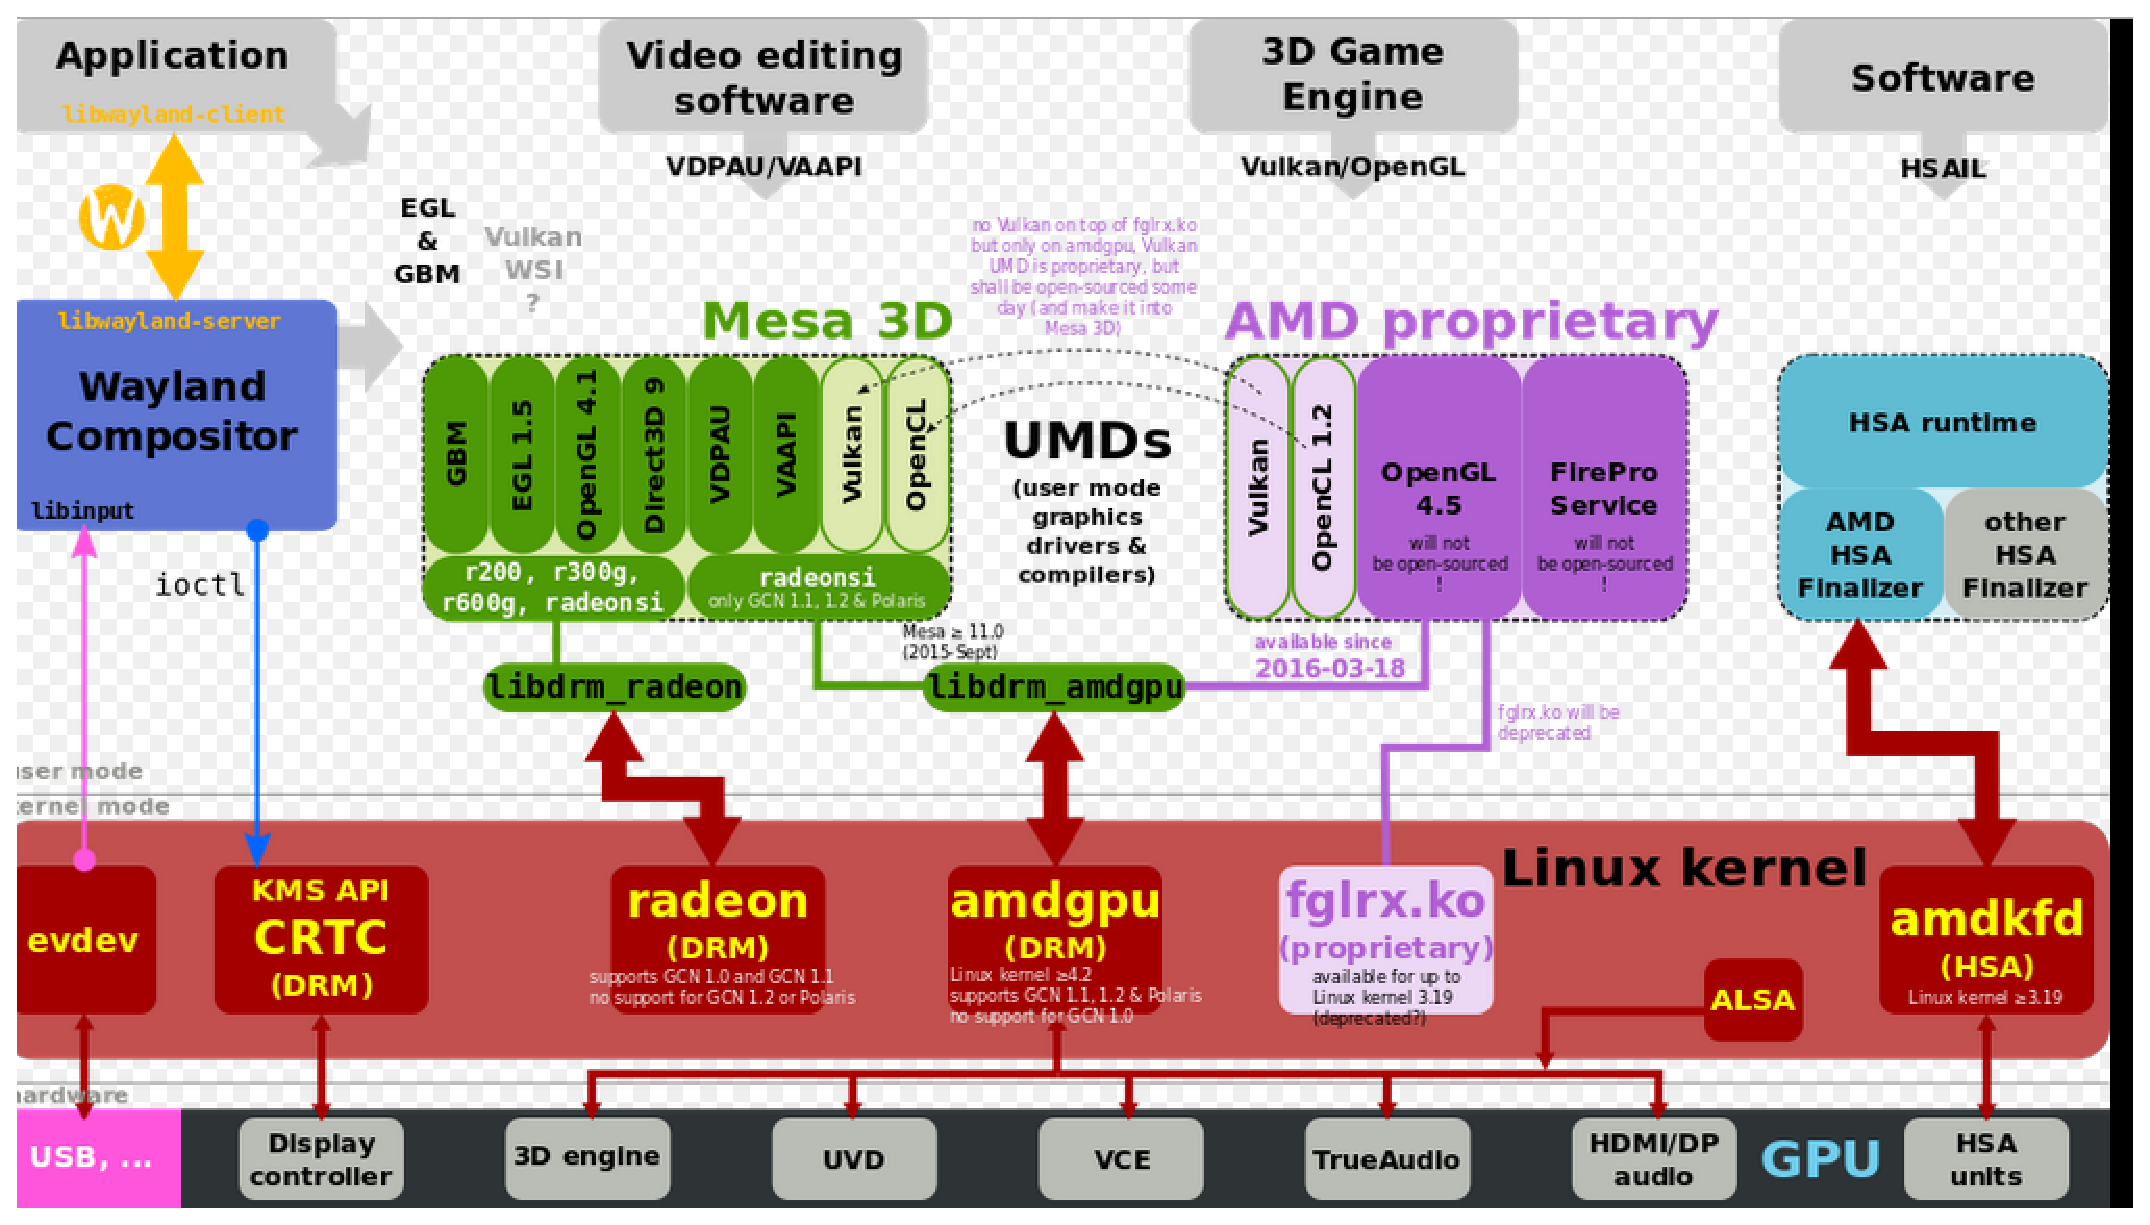
\includegraphics[width=14cm,height=9cm]{figures/chap01/linux-mesa}
  \caption{现代Linux图形栈与Mesa3D}
  \label{fig:linux-mesa}
\end{figure}

\subsection{Mesa3D版本信息}
为了匹配OpenGL的版本不断变化以及各大图形硬件厂商的图形设备不断更新,Mesa3D也一直不断的更新新的版本。到目前为止最新的Mesa3D版本为2016年3月更新的Version 11.2,详细版本更新信息以及支持的OpenGL版本见附录\ref{cha:Mesa3D-History-Version}
